In this chapter, we discuss our working pipeline and system architecture in details.  Generally, our system takes a speech note, textual description or numerical attributes as an input. It processes the input description and outputs the initial human face portrait that corresponds to the given description. Afterwards, the user is allowed to manually control some facial attributes and morphological features and to rotate the face and render it in multiple poses. In the first section, we give an overview about the system. Then, we discuss the system architecture in the second section. In the subsequent sections, each module implementation is discussed in details.

\subsection{Overview and Assumptions}

As mentioned above, our system basically enables the user to describe a human face in words or using numerical values and turns it into a full human face portrait that can be manipulated and rendered in multiple poses. The system relies heavily on generative models and text processing, both are iteratively designed to obtain the required results. The overall flow can be described as follows :
\begin{itemize}
    \item The input speech notes are translated to text.
    \item The textual description (extracted from speech input or manually entered) is processed to extract the numerical values of the required facial features.
    \item The numerical values are used generate a face embedding vector that encodes the facial attributes in low dimensional space ($512D$).
    \item A generative model is specifically designed to translate from the low dimensional embedding into the full face portrait ($1024X1024$).
    \item The generated face portrait can be further refined by navigating the face embedding space and re-generating the face portrait.
    \item Once the user settles on the final face portrait, the system can render that face in multiple poses to provide further identification.
\end{itemize}

The previous flow provides a very versatile framework to generate face portrait and adjust it to your liking. However, there is an extremely large number of facial attributes and morphological features to describe a human face. Consequently, we have to choose a descriptive subset of these attributes to consider in the face description. We consider $32$ facial attributes for face description, which are listed as follows :
\begin{itemize}
    \item Overall face :
    \begin{itemize}
        \item Gender : Male / Female.
        \item Age : Young / Old.
        \item Thickness : Chubby / Slim.
        \item Shape : Oval / Circular.
        \item Skin Color : Black / White.
        \item Cheeks : Normal / Rosy.
    \end{itemize}
    \item Eyes :
    \begin{itemize}
        \item Color : Black / Blue / Green / Brown.
        \item Width : Wide / Narrow.
        \item Eyebrows : Light / Bushy.
        \item Bags Under Eyes : On / Off.
    \end{itemize}
    \item Nose :
    \begin{itemize}
        \item Size : Big / Small.
        \item Pointy : On / Off.
    \end{itemize}
    \item Ears :
    \begin{itemize}
        \item Size : Big / Small.
    \end{itemize}
    \item Jaw :
    \begin{itemize}
        \item Mouth Size : Big / Small.
        \item Lips Size : Big / Small.
        \item Cheekbones : Low / High.
        \item Double Chin : On / Off.
    \end{itemize}
    \item Hair :
    \begin{itemize}
        \item Color : Black / Blonde / Brown / Red / Gray.
        \item Length : Tall / Short.
        \item Style : Straight / Curly / Receding Hairline / Bald / with Bangs.
    \end{itemize}
    \item Facial Hair :
    \begin{itemize}
        \item Beard / None.
    \end{itemize}
    \item Race :
    \begin{itemize}
        \item White / Black / Asian.
    \end{itemize}
    \item Accessories :
    \begin{itemize}
        \item Glasses : Sight / Sun.
        \item Makeup : On / Off.
        \item Lipstick : On / Off.
    \end{itemize}
\end{itemize}

\subsection{System Architecture}

Now, let's discuss our system architecture. The system consists of $7$ modules, $3$ core modules of the project and $4$ auxiliary modules.

\subsubsection{Block Diagram}

\begin{figure}[h]
    \centering
    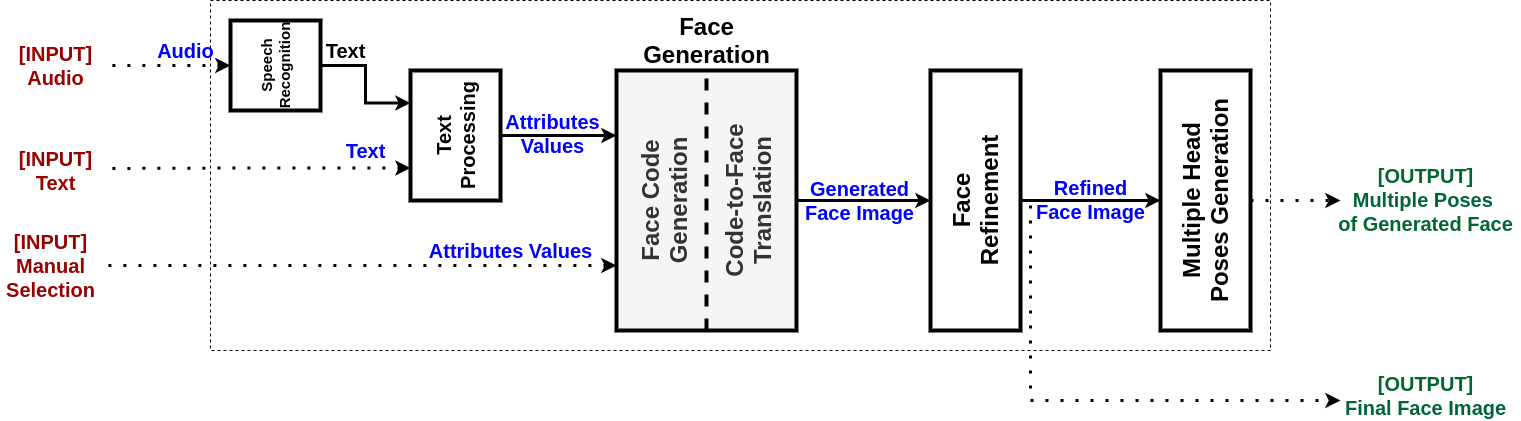
\includegraphics[width=\textwidth]{images/system-design.png}
    \caption{Block diagram of complete system architecture}
    \label{fig:system}
\end{figure}

\begin{figure}[h]
    \centering
    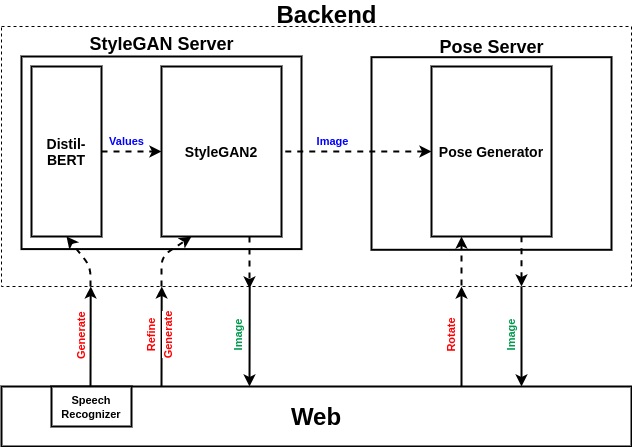
\includegraphics[width=0.8\textwidth]{images/app-design.png}
    \caption{Block diagram of application design}
    \label{fig:system}
\end{figure}

\subsection{Module 1 : Speech Recognition}
\subsubsection{Functional Description}
\subsubsection{Modular Decomposition}
\subsubsection{Design Constraints}
\subsubsection{Other Description}

\subsection{Module 2 : Text Processing}
\subsubsection{Functional Description}
\subsubsection{Modular Decomposition}
\subsubsection{Design Constraints}
\subsubsection{Other Description}

\subsection{Module 3 : Face Code Generation}
\subsubsection{Functional Description}
\subsubsection{Modular Decomposition}
\subsubsection{Design Constraints}
\subsubsection{Other Description}

\subsection{Module 4 : Code-to-Face Translation}
\subsubsection{Functional Description}
\subsubsection{Modular Decomposition}
\subsubsection{Design Constraints}
\subsubsection{Other Description}

\subsection{Module 5 : Face Refinement}
\subsubsection{Functional Description}
\subsubsection{Modular Decomposition}
\subsubsection{Design Constraints}
\subsubsection{Other Description}

\subsection{Module 6 : Multiple Head Poses Generation}
\subsubsection{Functional Description}
\subsubsection{Modular Decomposition}
\subsubsection{Design Constraints}
\subsubsection{Other Description}
